%=============================================================================
% Chapter 4: Two-Dimensional Arrays
%=============================================================================
\chapter{Two-Dimensional Arrays}
\label{ch:two-dimensional-arrays}

%-----------------------------------------------------------------------------
\section{Introduction to 2D Arrays}
\label{sec:intro-2d-arrays}
%-----------------------------------------------------------------------------

A one-dimensional array stores a single list of values. In many real-world
situations, however, data is naturally organised in a tabular
(row-and-column) format---exam scores for several students across multiple
subjects, pixel intensities in an image, or entries in a mathematical
matrix. For such cases C++ provides \emph{two-dimensional arrays}.

\begin{definitionbox}{Two-Dimensional Array}
A \textbf{two-dimensional (2D) array} is an array of arrays. It is a
collection of elements arranged in rows and columns, where each element is
accessed using \emph{two} indices: a \textbf{row index} and a
\textbf{column index}.
\end{definitionbox}

\begin{conceptbox}{Declaration Syntax}
\begin{verbatim}
    data-type  Array-name[Row-size][Col-size];
\end{verbatim}
\begin{itemize}
    \item \texttt{Row-size} --- the number of rows.
    \item \texttt{Col-size} --- the number of columns.
    \item The total number of elements is
          $\texttt{Row-size} \times \texttt{Col-size}$.
\end{itemize}
\end{conceptbox}

\paragraph{Examples.}

\begin{cppcode}
int a[10][10];   // 10 rows x 10 columns (100 elements)
int num[3][4];   //  3 rows x  4 columns ( 12 elements)
\end{cppcode}

\subsection*{Visualising a 2D Array}

The diagram below shows the layout of \texttt{int num[3][4]}. Rows are
numbered 0--2 and columns 0--3.

\begin{center}
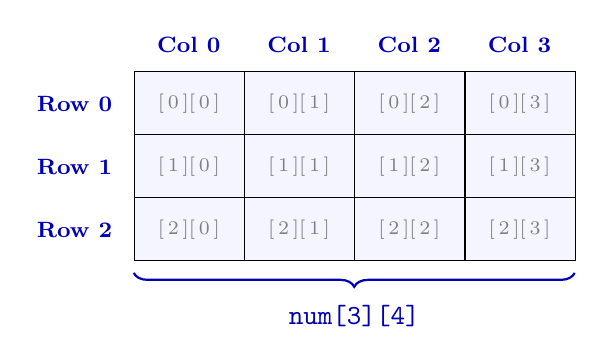
\begin{tikzpicture}[
    cell/.style={
        draw,
        minimum width=1.4cm,
        minimum height=0.8cm,
        anchor=south west,
        font=\small\ttfamily,
        fill=blue!4
    },
    hdr/.style={
        font=\footnotesize\bfseries,
        text=blue!70!black
    }
]
% Column headers
\foreach \j in {0,...,3} {
    \node[hdr] at (\j*1.4+0.7, 2.75) {Col \j};
}

% Row 2 (index 0 at top of diagram)
\node[hdr, anchor=east] at (-0.15, 2.0) {Row 0};
\foreach \j in {0,...,3} {
    \node[cell] at (\j*1.4, 1.6) {};
    \node[font=\scriptsize, gray] at (\j*1.4+0.7, 2.0) {[\,0\,][\,\j\,]};
}

% Row 1
\node[hdr, anchor=east] at (-0.15, 1.2) {Row 1};
\foreach \j in {0,...,3} {
    \node[cell] at (\j*1.4, 0.8) {};
    \node[font=\scriptsize, gray] at (\j*1.4+0.7, 1.2) {[\,1\,][\,\j\,]};
}

% Row 0
\node[hdr, anchor=east] at (-0.15, 0.4) {Row 2};
\foreach \j in {0,...,3} {
    \node[cell] at (\j*1.4, 0) {};
    \node[font=\scriptsize, gray] at (\j*1.4+0.7, 0.4) {[\,2\,][\,\j\,]};
}

% Array name brace
\draw[decorate,
      decoration={brace, amplitude=5pt, mirror},
      thick, blue!70!black]
    (0, -0.15) -- (5.6, -0.15)
    node[midway, below=8pt, font=\bfseries\ttfamily,
         text=blue!70!black] {num[3][4]};
\end{tikzpicture}
\end{center}

\begin{infobox}{Memory Layout}
Although we visualise a 2D array as a grid, in memory the elements are
stored in \emph{row-major order}: all elements of row~0 come first,
followed by all elements of row~1, and so on.

\medskip
\begin{center}
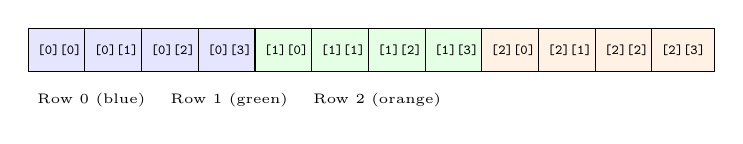
\begin{tikzpicture}[
    cell/.style={
        draw, minimum width=0.72cm, minimum height=0.55cm,
        font=\tiny\ttfamily, fill=white, anchor=south west
    }
]
\foreach \i/\lbl/\clr in {%
    0/{[0][0]}/blue!10, 1/{[0][1]}/blue!10,
    2/{[0][2]}/blue!10, 3/{[0][3]}/blue!10,
    4/{[1][0]}/green!10, 5/{[1][1]}/green!10,
    6/{[1][2]}/green!10, 7/{[1][3]}/green!10,
    8/{[2][0]}/orange!10, 9/{[2][1]}/orange!10,
    10/{[2][2]}/orange!10, 11/{[2][3]}/orange!10%
} {
    \node[cell, fill=\clr] at (\i*0.72, 0) {\lbl};
}
\node[font=\tiny, anchor=west] at (0, -0.35)
    {Row 0 (blue) \quad Row 1 (green) \quad Row 2 (orange)};
\end{tikzpicture}
\end{center}
\end{infobox}

%-----------------------------------------------------------------------------
\section{Initialising 2D Arrays}
\label{sec:init-2d-arrays}
%-----------------------------------------------------------------------------

A two-dimensional array can be initialised at the point of declaration using
nested brace-enclosed lists---one inner list per row:

\begin{cppcode}
int a[2][3] = {
    {1, 2, 3},   // row 0
    {4, 5, 6}    // row 1
};
\end{cppcode}

\subsection*{Resulting Layout}

The table below shows the values stored in each position after the
initialisation above.

\begin{center}
\renewcommand{\arraystretch}{1.3}
\begin{tabular}{@{} c ccc @{}}
\toprule
    & \textbf{Col 0} & \textbf{Col 1} & \textbf{Col 2} \\
\midrule
\textbf{Row 0} & 1 & 2 & 3 \\
\textbf{Row 1} & 4 & 5 & 6 \\
\bottomrule
\end{tabular}
\end{center}

\begin{warningbox}{Row Size Can Be Omitted --- Column Size Cannot}
When an initialiser list is provided, the compiler can deduce the number
of rows, so you may write
\texttt{int a[][3] = \{\{1,2,3\},\{4,5,6\}\};}. However, the
\emph{column} size must always be specified explicitly.
\end{warningbox}

%-----------------------------------------------------------------------------
\section{Reading, Writing, and Processing 2D Arrays}
\label{sec:rwp-2d-arrays}
%-----------------------------------------------------------------------------

Processing a 2D array requires \emph{nested loops}: the outer loop iterates
over the rows, and the inner loop iterates over the columns (or vice versa).

%--------------------------------------------------------------------
\subsection{Example 1: Read and Print a
            3\texorpdfstring{\texttimes}{x}5 Array}

\textbf{Problem.} Read a $3 \times 5$ array of integers from the user,
then print all elements.

\begin{cppcode}
#include <iostream>
using namespace std;

int main() {
    int arr[3][5];

    // Reading
    cout << "Enter 15 integers (3 rows x 5 cols):"
         << endl;
    for (int i = 0; i < 3; i++) {
        for (int j = 0; j < 5; j++) {
            cin >> arr[i][j];
        }
    }

    // Printing
    cout << "Array elements:" << endl;
    for (int i = 0; i < 3; i++) {
        for (int j = 0; j < 5; j++) {
            cout << arr[i][j] << "\t";
        }
        cout << endl;
    }

    return 0;
}
\end{cppcode}

\textbf{Sample run:}
\begin{verbatim}
Enter 15 integers (3 rows x 5 cols):
1 2 3 4 5 6 7 8 9 10 11 12 13 14 15
Array elements:
1       2       3       4       5
6       7       8       9       10
11      12      13      14      15
\end{verbatim}

%--------------------------------------------------------------------
\subsection{Example 2: Read, Sum, and Print a
            4\texorpdfstring{\texttimes}{x}4 Array}

\textbf{Problem.} Read a $4 \times 4$ array, compute the summation of
all elements, and print the array together with the total.

\begin{cppcode}
#include <iostream>
using namespace std;

int main() {
    int arr[4][4];
    int sum = 0;

    cout << "Enter 16 integers (4 x 4):" << endl;
    for (int i = 0; i < 4; i++) {
        for (int j = 0; j < 4; j++) {
            cin >> arr[i][j];
        }
    }

    // Print and accumulate
    cout << "Array elements:" << endl;
    for (int i = 0; i < 4; i++) {
        for (int j = 0; j < 4; j++) {
            cout << arr[i][j] << "\t";
            sum += arr[i][j];
        }
        cout << endl;
    }

    cout << "Summation of all elements = "
         << sum << endl;

    return 0;
}
\end{cppcode}

\textbf{Sample run:}
\begin{verbatim}
Enter 16 integers (4 x 4):
1 2 3 4 5 6 7 8 9 10 11 12 13 14 15 16
Array elements:
1       2       3       4
5       6       7       8
9       10      11      12
13      14      15      16
Summation of all elements = 136
\end{verbatim}

%--------------------------------------------------------------------
\subsection{Example 3: Summation of Each Row}

\textbf{Problem.} Read a $3 \times 4$ array and compute the summation
of each row separately.

\begin{cppcode}
#include <iostream>
using namespace std;

int main() {
    int arr[3][4];

    cout << "Enter 12 integers (3 x 4):" << endl;
    for (int i = 0; i < 3; i++) {
        for (int j = 0; j < 4; j++) {
            cin >> arr[i][j];
        }
    }

    for (int i = 0; i < 3; i++) {
        int rowSum = 0;
        for (int j = 0; j < 4; j++) {
            rowSum += arr[i][j];
        }
        cout << "Sum of row " << i
             << " = " << rowSum << endl;
    }

    return 0;
}
\end{cppcode}

\textbf{Sample run:}
\begin{verbatim}
Enter 12 integers (3 x 4):
1 2 3 4 5 6 7 8 9 10 11 12
Sum of row 0 = 10
Sum of row 1 = 26
Sum of row 2 = 42
\end{verbatim}

\begin{importantbox}{Row Summation Pattern}
To sum each row independently, reset the accumulator variable
(\texttt{rowSum}) to zero at the \emph{beginning} of each iteration of
the outer loop. This ensures that each row's total is computed from
scratch.
\end{importantbox}

%--------------------------------------------------------------------
\subsection{Example 4: Replace a Specific Value}

\textbf{Problem.} Read a $3 \times 4$ array and replace every
occurrence of the value~5 with~0.

\begin{cppcode}
#include <iostream>
using namespace std;

int main() {
    int arr[3][4];

    cout << "Enter 12 integers (3 x 4):" << endl;
    for (int i = 0; i < 3; i++) {
        for (int j = 0; j < 4; j++) {
            cin >> arr[i][j];
        }
    }

    // Replace 5 with 0
    for (int i = 0; i < 3; i++) {
        for (int j = 0; j < 4; j++) {
            if (arr[i][j] == 5) {
                arr[i][j] = 0;
            }
        }
    }

    // Print the modified array
    cout << "Array after replacement:" << endl;
    for (int i = 0; i < 3; i++) {
        for (int j = 0; j < 4; j++) {
            cout << arr[i][j] << "\t";
        }
        cout << endl;
    }

    return 0;
}
\end{cppcode}

\textbf{Sample run:}
\begin{verbatim}
Enter 12 integers (3 x 4):
1 5 3 4 5 6 5 8 9 10 5 12
Array after replacement:
1       0       3       4
0       6       0       8
9       10      0       12
\end{verbatim}

%--------------------------------------------------------------------
\subsection{Example 5: Adding Two 2D Arrays}

\textbf{Problem.} Read two $3 \times 4$ arrays and compute their
element-wise sum into a third array.

\begin{cppcode}
#include <iostream>
using namespace std;

int main() {
    int a[3][4], b[3][4], c[3][4];

    cout << "Enter first array (3 x 4):" << endl;
    for (int i = 0; i < 3; i++)
        for (int j = 0; j < 4; j++)
            cin >> a[i][j];

    cout << "Enter second array (3 x 4):" << endl;
    for (int i = 0; i < 3; i++)
        for (int j = 0; j < 4; j++)
            cin >> b[i][j];

    // Element-wise addition
    for (int i = 0; i < 3; i++)
        for (int j = 0; j < 4; j++)
            c[i][j] = a[i][j] + b[i][j];

    // Print the result
    cout << "Sum of the two arrays:" << endl;
    for (int i = 0; i < 3; i++) {
        for (int j = 0; j < 4; j++) {
            cout << c[i][j] << "\t";
        }
        cout << endl;
    }

    return 0;
}
\end{cppcode}

\textbf{Sample run:}
\begin{verbatim}
Enter first array (3 x 4):
1 2 3 4 5 6 7 8 9 10 11 12
Enter second array (3 x 4):
10 20 30 40 50 60 70 80 90 100 110 120
Sum of the two arrays:
11      22      33      44
55      66      77      88
99      110     121     132
\end{verbatim}

%--------------------------------------------------------------------
\subsection{Example 6: Converting a 2D Array to a 1D Array}

\textbf{Problem.} Given a $3 \times 4$ array, copy all of its elements
into a one-dimensional array of size~12.

\begin{cppcode}
#include <iostream>
using namespace std;

int main() {
    int arr2D[3][4];
    int arr1D[12];

    cout << "Enter 12 integers (3 x 4):" << endl;
    for (int i = 0; i < 3; i++)
        for (int j = 0; j < 4; j++)
            cin >> arr2D[i][j];

    // Flatten 2D -> 1D
    int k = 0;
    for (int i = 0; i < 3; i++) {
        for (int j = 0; j < 4; j++) {
            arr1D[k] = arr2D[i][j];
            k++;
        }
    }

    // Print the 1D array
    cout << "1D array: ";
    for (int i = 0; i < 12; i++) {
        cout << arr1D[i] << " ";
    }
    cout << endl;

    return 0;
}
\end{cppcode}

\textbf{Sample run:}
\begin{verbatim}
Enter 12 integers (3 x 4):
1 2 3 4 5 6 7 8 9 10 11 12
1D array: 1 2 3 4 5 6 7 8 9 10 11 12
\end{verbatim}

\begin{conceptbox}{Flattening a 2D Array}
Converting a 2D array with $R$ rows and $C$ columns into a 1D array of
size $R \times C$ is called \textbf{flattening}. The element at position
\texttt{[i][j]} in the 2D array maps to index $i \times C + j$ in the
1D array. Equivalently, you can use a simple counter variable \texttt{k}
that increments with every element, as shown above.
\end{conceptbox}

%-----------------------------------------------------------------------------
\section{Matrix Diagonal Operations}
\label{sec:diagonal-operations}
%-----------------------------------------------------------------------------

When a 2D array represents a square matrix (same number of rows and
columns), several special index relationships identify important regions
of the matrix.

\begin{definitionbox}{Diagonal and Triangular Regions}
For an $n \times n$ square matrix with row index $i$ and column index $j$
(both starting from~0):
\begin{itemize}
    \item \textbf{Main diagonal:} elements where $i = j$.
    \item \textbf{Secondary diagonal:} elements where
          $i + j = n - 1$.
    \item \textbf{Upper triangle:} elements where $i < j$
          (above the main diagonal).
    \item \textbf{Lower triangle:} elements where $i > j$
          (below the main diagonal).
\end{itemize}
\end{definitionbox}

\subsection*{Visual Reference --- 3\texorpdfstring{\texttimes}{x}3
             Matrix}

The following colour-coded diagram illustrates these regions for a
$3 \times 3$ matrix. Each cell shows the index condition it satisfies.

\begin{center}
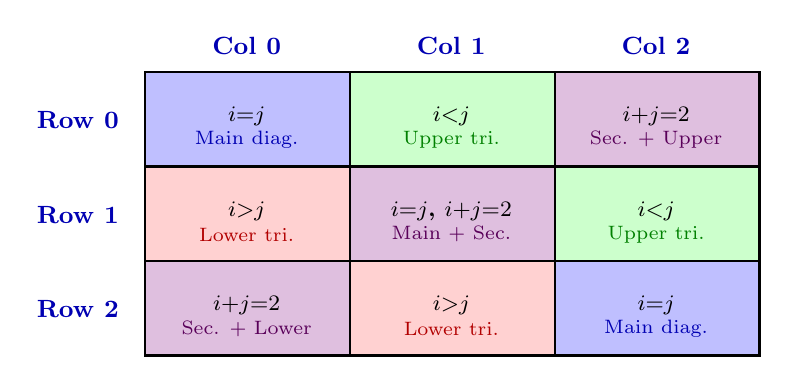
\begin{tikzpicture}[
    cell/.style={
        draw, thick,
        minimum width=2.6cm,
        minimum height=1.2cm,
        anchor=south west,
        font=\small
    },
    main/.style={cell, fill=blue!25},
    secondary/.style={cell, fill=orange!35},
    upper/.style={cell, fill=green!20},
    lower/.style={cell, fill=red!18},
    both/.style={cell, fill=violet!25},
    hdr/.style={font=\small\bfseries, text=blue!70!black}
]
% Column headers
\foreach \j in {0,1,2} {
    \node[hdr] at (\j*2.6+1.3, 3.95) {Col \j};
}

% ------- Row 0 (top, y=2.4) -------
\node[hdr, anchor=east] at (-0.2, 3.0) {Row 0};
% (0,0): i==j => Main diagonal
\node[main] at (0, 2.4) {};
\node[font=\footnotesize\bfseries] at (1.3, 3.05) {$i{=}j$};
\node[font=\scriptsize, text=blue!70!black] at (1.3, 2.75)
    {Main diag.};

% (0,1): i<j => Upper triangle
\node[upper] at (2.6, 2.4) {};
\node[font=\footnotesize\bfseries] at (3.9, 3.05) {$i{<}j$};
\node[font=\scriptsize, text=green!50!black] at (3.9, 2.75)
    {Upper tri.};

% (0,2): i<j AND i+j==2 => Secondary + Upper
\node[both] at (5.2, 2.4) {};
\node[font=\footnotesize\bfseries] at (6.5, 3.05)
    {$i{+}j{=}2$};
\node[font=\scriptsize, text=violet!70!black] at (6.5, 2.75)
    {Sec. + Upper};

% ------- Row 1 (middle, y=1.2) -------
\node[hdr, anchor=east] at (-0.2, 1.8) {Row 1};
% (1,0): i>j => Lower triangle
\node[lower] at (0, 1.2) {};
\node[font=\footnotesize\bfseries] at (1.3, 1.85) {$i{>}j$};
\node[font=\scriptsize, text=red!70!black] at (1.3, 1.55)
    {Lower tri.};

% (1,1): i==j AND i+j==2 => Main + Secondary
\node[both] at (2.6, 1.2) {};
\node[font=\footnotesize\bfseries] at (3.9, 1.85)
    {$i{=}j$, $i{+}j{=}2$};
\node[font=\scriptsize, text=violet!70!black] at (3.9, 1.55)
    {Main + Sec.};

% (1,2): i<j => Upper triangle
\node[upper] at (5.2, 1.2) {};
\node[font=\footnotesize\bfseries] at (6.5, 1.85) {$i{<}j$};
\node[font=\scriptsize, text=green!50!black] at (6.5, 1.55)
    {Upper tri.};

% ------- Row 2 (bottom, y=0) -------
\node[hdr, anchor=east] at (-0.2, 0.6) {Row 2};
% (2,0): i>j AND i+j==2 => Secondary + Lower
\node[both] at (0, 0) {};
\node[font=\footnotesize\bfseries] at (1.3, 0.65)
    {$i{+}j{=}2$};
\node[font=\scriptsize, text=violet!70!black] at (1.3, 0.35)
    {Sec. + Lower};

% (2,1): i>j => Lower triangle
\node[lower] at (2.6, 0) {};
\node[font=\footnotesize\bfseries] at (3.9, 0.65) {$i{>}j$};
\node[font=\scriptsize, text=red!70!black] at (3.9, 0.35)
    {Lower tri.};

% (2,2): i==j => Main diagonal
\node[main] at (5.2, 0) {};
\node[font=\footnotesize\bfseries] at (6.5, 0.65) {$i{=}j$};
\node[font=\scriptsize, text=blue!70!black] at (6.5, 0.35)
    {Main diag.};
\end{tikzpicture}
\end{center}

\medskip

% Legend as a compact table
\begin{center}
\renewcommand{\arraystretch}{1.2}
\begin{tabular}{@{} >{\centering\arraybackslash}p{1.8cm}
                    >{\centering\arraybackslash}p{1.8cm}
                    >{\centering\arraybackslash}p{1.8cm}
                    >{\centering\arraybackslash}p{1.8cm}
                    >{\centering\arraybackslash}p{1.8cm} @{}}
\toprule
\colorbox{blue!25}{\strut\hspace{8mm}} &
\colorbox{orange!35}{\strut\hspace{8mm}} &
\colorbox{green!20}{\strut\hspace{8mm}} &
\colorbox{red!18}{\strut\hspace{8mm}} &
\colorbox{violet!25}{\strut\hspace{8mm}} \\
\footnotesize Main diag. &
\footnotesize Sec.\ diag. &
\footnotesize Upper tri. &
\footnotesize Lower tri. &
\footnotesize Overlap \\
\footnotesize $i = j$ &
\footnotesize $i{+}j = n{-}1$ &
\footnotesize $i < j$ &
\footnotesize $i > j$ &
\footnotesize (both) \\
\bottomrule
\end{tabular}
\end{center}

\medskip

The following summary table also maps every cell of a $3\times 3$ matrix
to its region:

\begin{center}
\renewcommand{\arraystretch}{1.3}
\begin{tabular}{@{} c ccc @{}}
\toprule
    & \textbf{Col 0} & \textbf{Col 1} & \textbf{Col 2} \\
\midrule
\textbf{Row 0}
    & $a_{00}$\;\textsuperscript{main}
    & $a_{01}$\;\textsuperscript{upper}
    & $a_{02}$\;\textsuperscript{sec., upper} \\
\textbf{Row 1}
    & $a_{10}$\;\textsuperscript{lower}
    & $a_{11}$\;\textsuperscript{main, sec.}
    & $a_{12}$\;\textsuperscript{upper} \\
\textbf{Row 2}
    & $a_{20}$\;\textsuperscript{sec., lower}
    & $a_{21}$\;\textsuperscript{lower}
    & $a_{22}$\;\textsuperscript{main} \\
\bottomrule
\end{tabular}
\end{center}

%--------------------------------------------------------------------
\subsection{Example 7: Replace Main Diagonal with Zero}

\textbf{Problem.} Read a $4 \times 4$ matrix and replace all elements
on the main diagonal with zero, then print the result.

\begin{cppcode}
#include <iostream>
using namespace std;

int main() {
    int arr[4][4];

    cout << "Enter 16 integers (4 x 4):" << endl;
    for (int i = 0; i < 4; i++)
        for (int j = 0; j < 4; j++)
            cin >> arr[i][j];

    // Replace main diagonal elements with 0
    for (int i = 0; i < 4; i++) {
        arr[i][i] = 0;   // main diagonal: i == j
    }

    // Print the modified matrix
    cout << "Matrix after replacing diagonal:"
         << endl;
    for (int i = 0; i < 4; i++) {
        for (int j = 0; j < 4; j++) {
            cout << arr[i][j] << "\t";
        }
        cout << endl;
    }

    return 0;
}
\end{cppcode}

\textbf{Sample run:}
\begin{verbatim}
Enter 16 integers (4 x 4):
1 2 3 4 5 6 7 8 9 10 11 12 13 14 15 16
Matrix after replacing diagonal:
0       2       3       4
5       0       7       8
9       10      0       12
13      14      15      0
\end{verbatim}

\begin{infobox}{Accessing the Main Diagonal Efficiently}
Since main-diagonal elements satisfy $i = j$, you only need a
\emph{single} loop---not nested loops---to visit them all:
\texttt{for (int i = 0; i < n; i++) arr[i][i] = 0;}.
\end{infobox}

%--------------------------------------------------------------------
\subsection{Example 8: Square Root of Array Elements}

\textbf{Problem.} Read a $3 \times 3$ array of \texttt{double} values
and print the square root of each element.

\begin{cppcode}
#include <iostream>
#include <cmath>
using namespace std;

int main() {
    double arr[3][3];

    cout << "Enter 9 values (3 x 3):" << endl;
    for (int i = 0; i < 3; i++)
        for (int j = 0; j < 3; j++)
            cin >> arr[i][j];

    cout << "Square roots:" << endl;
    for (int i = 0; i < 3; i++) {
        for (int j = 0; j < 3; j++) {
            cout << sqrt(arr[i][j]) << "\t";
        }
        cout << endl;
    }

    return 0;
}
\end{cppcode}

\textbf{Sample run:}
\begin{verbatim}
Enter 9 values (3 x 3):
4 9 16 25 36 49 64 81 100
Square roots:
2       3       4
5       6       7
8       9       10
\end{verbatim}

\begin{warningbox}{Negative Values under \texttt{sqrt}}
The \texttt{sqrt} function from \texttt{<cmath>} returns \texttt{NaN}
(Not a Number) when given a negative argument. In a robust program you
should validate that each value is non-negative before computing its
square root.
\end{warningbox}

%--------------------------------------------------------------------
\subsection{Example 9: Sum of Main and Secondary Diagonals}

\textbf{Problem.} Read a $4 \times 4$ integer matrix and compute:
\begin{enumerate}
    \item The sum of the \emph{main diagonal} elements.
    \item The sum of the \emph{secondary diagonal} elements.
\end{enumerate}

\begin{cppcode}
#include <iostream>
using namespace std;

int main() {
    int arr[4][4];
    int mainSum = 0, secSum = 0;
    int n = 4;

    cout << "Enter 16 integers (4 x 4):" << endl;
    for (int i = 0; i < n; i++)
        for (int j = 0; j < n; j++)
            cin >> arr[i][j];

    for (int i = 0; i < n; i++) {
        mainSum += arr[i][i];
        secSum  += arr[i][n - 1 - i];
    }

    cout << "Sum of main diagonal      = "
         << mainSum << endl;
    cout << "Sum of secondary diagonal  = "
         << secSum  << endl;

    return 0;
}
\end{cppcode}

\textbf{Sample run:}
\begin{verbatim}
Enter 16 integers (4 x 4):
1 2 3 4 5 6 7 8 9 10 11 12 13 14 15 16
Sum of main diagonal      = 34
Sum of secondary diagonal  = 34
\end{verbatim}

\begin{importantbox}{Diagonal Summation in a Single Loop}
Both diagonal sums can be computed in a single loop of $n$ iterations.
\begin{itemize}
    \item For the main diagonal, the column index equals the row
          index: use \texttt{arr[i][i]}.
    \item For the secondary diagonal, the column index is
          \texttt{n\,-\,1\,-\,i}: use \texttt{arr[i][n-1-i]}.
\end{itemize}
Note: in a matrix with an odd dimension, the centre element belongs to
\emph{both} diagonals. If you need the combined sum without
double-counting, subtract that centre element once.
\end{importantbox}
